% class definitions
\documentclass[12pt]{article}
\usepackage[ngerman,english]{babel}
\setlength{\parindent}{0em} 

% Packages

\usepackage[utf8]{inputenc}
\usepackage[ngerman]{babel}
\usepackage[T1]{fontenc}
\usepackage{graphicx}
\usepackage{lmodern}
\usepackage{tabto}
\usepackage{listings}
\usepackage{quoting} %
\usepackage{lipsum}
\usepackage[left, pagewise, edtable]{lineno}
\quotingsetup{font={itshape}, leftmargin=2em, rightmargin=0in, vskip=1ex}
\usepackage{framed} 
\usepackage{xcolor}
\usepackage{tcolorbox}
\usepackage{xcolor} 
\colorlet{shadecolor}{gray!25}
\definecolor{mshadecolor}{rgb}{0.7421875,0.7421875,0.7421875}

%myshaded
\newenvironment{myshaded}{\colorlet{shadecolor}{lightgray}\color{black}\begin{shaded}\begin{internallinenumbers}}{\end{internallinenumbers}\end{shaded}}

%bibtext
\usepackage[backend=biber, style=authoryear]{biblatex}
\addbibresource{quellen.bib}


% Front page

\title{\small{WPM}\\\vspace{3mm}\Large{Hacking mit Python\\\small{Projektdokumentation}}}
\author{ \small{verfasst von}\\ Moritz Rupp}
\date{Sommersemester 2022}

%Document start 
\begin{document}



\maketitle
\newpage
\tableofcontents
\newpage

\begin{abstract}
\noindent In dem Modul 'Hacking mit Python' ist es Aufgabe verschiedene Services wie ein HTTP Server und SSH automatisiert anhand der Programmiersprache Python anzugreifen und zu kompromitieren.\\ Hierfür können verschiedene Frameworks und Tools genutzt werden. 
\end{abstract}

\section{Einleitung}
Anwendungen wie Webserver sind häufig der zentrale und angreifsbarste Teil einer digitalen Infrastrustur. So werden hier meist nicht nur harmlose Html Dokumente abgerufen, sondern häufig auch Sicherheitsrelevante Dienste und Dateien gehosted. Dies können Zugänge der Schnittstelle, unverschlüsselte Nutzerdaten oder viele weitere sensitive Informationen sein.
\\
Ziel dieses Projektes ist es die angreifbare Infrastrustur in Form des Webserver bereitzustellen und diesen anschließend anhand einer in Python programmierten Software anzugreifen.
Der Angriff soll im ersten Schritt alle Inhalte des Opfer-Servers aufspüren und herunterladen. Anschließend sollten über den Browser alle Seiten automatisiert besucht und die Funktionalität genutzt werden.
Des weiteren ist eine in der Infrastrustur bereitgestellte Schnittstelle wie SSH anhand eines Wörterbuch-Angriffs zu kompromitieren. Abschließend soll mit den erlangten Zugangsdaten eine Schadsoftware auf den Opfer-Server geladen werden, mit dieser ein defacement der gehosteten Webseite umgesetzt werden kann.\\
Dieses Dokument beleuchtet die Umsetzung und Implementierung der einzelnen Schritte. 

\newpage
\section{Infrastrustur}
\subsection{Opfer-Server}
Der Opfer-Server soll ein Http-Server mit angreifbarer Webanwendung und Schnittstelle sein. Hierfür kommen etliche Frameworks und Distributionen wie Apache und xampp in Frage.
Aufrund der Anforderungen habe ich mich für eine Node Anwendung in einem Docker Container entschieden.
Container sind eine leichtgewichtige Art von Virtualisierung auf Betriebssystemebene. Dies kann genutzt werden um eine Anwendung mitsamt ihren Abhängigkeiten als eine abgeschlossene Einheit zu verpacken und zu betrieben. Dies bietet Vorteile wie Plattformunabhängigkeit und einfache Ausfürbarkeit. In diesem Fall wird ein node Web-Server mitsamt SSH Service aufgesetzt.\\
Das Packet aus Anwendung und Abhängigkeiten
nennt man auch Container-Image. Dies kann anhand des Dockerfiles erzeugt werden. Das Dockerfile enthält alle Instruktionen die zur Erstellung des Images benötigt werden.  \\
\begin{shaded}
\begin{internallinenumbers}
FROM ubuntu:latest

RUN apt update \&\& apt install  openssh-server sudo -y

RUN apt install git -y

RUN apt install nodejs -y

RUN apt install npm -y

RUN npm install express

RUN npm install better-sqlite3

RUN npm install morgan

RUN echo "PermitRootLogin yes"\>etc/ssh/sshd\_config

RUN  echo 'root:root' | chpasswd

RUN service ssh start

EXPOSE 22

RUN git clone https://github.com/mauriceKalevra/Web2-Projekt.git

WORKDIR Web2-Projekt

RUN npm install

RUN echo  "/usr/sbin/sshd -D \& node app.js">entrypoint.sh

RUN chmod 700 entrypoint.sh

CMD ./entrypoint.sh
\end{internallinenumbers}
\end{shaded}
\begin{center}
 Codebeispiel 1: Dockerfile des Http-SSH-Servers
\end{center}
Ein Container wird stets auf einem Base Image aufgebaut. Dieses dient als Fundament für alle folge Instruktionen und enthält je nach Image ein grundlegendes Dateisystem sowie vorinstallierte Software.\\
In Zeile 1(vgl. Codebeispiel 1) wird als Base Image Ubuntu deklariert. 
Anschließend werden verschiedene Dienste wie openssh, git, nodejs sowie einige npm Packete installiert.
In Zeile 10 wird das root Passwort für die Schnittstelle des Webservers bzw. Containers festgelegt. Die eigentliche Webanwendung wird in Zeile 13 als ein Repository durch git heruntergeladen und ins Zeile 15 installiert. In Zeile 16 wird das Kommando zum starten des SSH Dienstes und der Node Anwendung in ein Bash-Skript geschrieben, um dieses anschließend ausführbar zu machen und in Zeile 18 zu starten.\\
Mit \colorbox{mshadecolor}{\parbox{0.46\textwidth}{Docker build -t victim-http-server .}} wird aus dem Dockerfile ein Image erstellt. Alternativ kann das kompilierte Image auch über Dockerhub mit \colorbox{mshadecolor}{\parbox{0.58\textwidth}{Docker pull mauriceKalevra/ssh-node-server}} geladen werden. Dieses kann nun mit \colorbox{mshadecolor}{\parbox{0.51\textwidth}{Docker run -p 22:22 victim-http-server}} gestartet werden. Nun läuft der HTTP Server und die Webanwendung ist im Browser unter
\colorbox{mshadecolor}{\parbox{0.20\textwidth}{173.17.0.2:1337}} einsehbar. Des weiteren ist eine Admin Schnittstelle über \colorbox{mshadecolor}{\parbox{0.26\textwidth}{ssh root@173.17.0.2}} erreichbar.
\subsubsection{Webanwendung}
Als Webanwendung dient ein Projekt aus einem früheren Semester. Dort war es Aufgabe eine Dynamische Webseite unter anderem mit einem NodeJs backend zu entwickeln. In der Anwendung 'Real-Estate Albsig' ist es möglich Immobilien Angebote zu Inserieren, suchen und einzusehen. Die Inserate und gesuche werden zudem auf dem Webserver in einer sqlite Datenbank gespeichert. Die Anwendung enthält mehrere Html/Css Dokumente, Ordner für Bilder, Javaskript Dateien und die Datenbank welche in einem Isolierten Verzeichniss liegt. Des weiteren exisitiert ein Dockerfile mit entsprechenden Konfigurationen.          
\newpage
\section{Angriffe auf den Opfer-Server}
\subsection{Spider-Angriff}
Bei einem Spider Angriff ist es Ziel alle Ressourcen eines Webservers aufzusprüren und Herunterzuladen.
Folgendes Codebeispiel versucht in einer Funktion mit Hilfe des Moduls requests alle Verzeichnisse und Dateien auf einem Webserver ausfindig zu machen.

Erster Ansatz war es mit hilfe der python Biblothek 'Beautifullsoup' alle html Dokumente ausfindig zu machen.
Hierbei wird auch mit dem python modul 'requests' gearbeitet. Dieses nimmt als Parameter eine url entgegen und holt über ein http request das html Dokument ein(vgl. Zeile 2). Dieses wird nun mit Beautifullsoup geparsed(vgl. Zeile 3). In Zeile 5 werden nun in einer for schleife alle html hyperlink-tags gefunden, in Zeile 6 auf die urls minimiert(vgl. Zeile 7) und schließlich ausgegeben. Die einfache Funktion findet nahezu alle html Seiten.
\begin{center}
 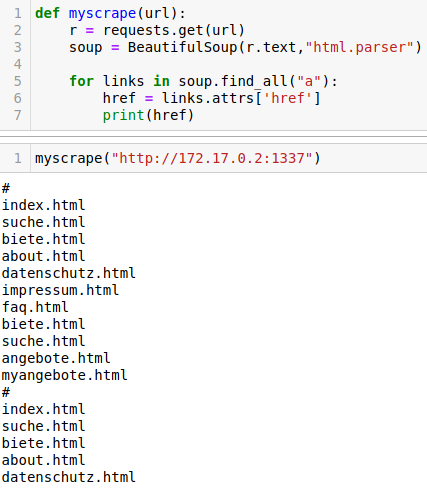
\includegraphics[scale=0.5]{data/scrapemy.png}
\end{center}
\begin{center}
 Codebeispiel 2: Python Funktion myscrape
\end{center}
\newpage
Um alle weiteren Html Dokumente sowie Verzeichhnisse und Bilder zu finden verwendet die Funktion 'mygobuster' Wörterlisten und Rekursion.
\begin{center}
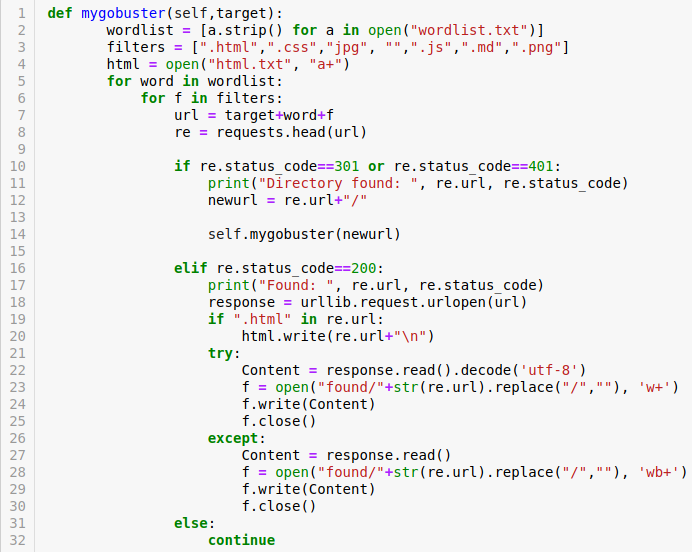
\includegraphics[scale=0.5]{data/mygobuster.png}
Codebeispiel 3: Python Funktion mygobuster
\end{center}
Hierbei wird in Zeile 2 eine Wörterliste mit üblichen Nodejs-Verzeichnis und Dateinamen anhand einer List Comprehension eingelesen und entsprechend formatiert.
In der Liste 'filters' befinden sich Dateiendungen nach denen gesucht werden soll. Nun wird über beide Listen iteriert und diese mit der url des Opfer-Servers verknüpft(vgl. Zeile 7) und dem Modul request übergeben(vgl. Zeile 8). Mit diesem ist es möglich Http Funktionalitäten zu nutzen. So wird ein Http request an den Opfer-Server geschickt und der Response code ausgelesen(vgl. Zeile 10). Gibt der Webserver den Statuscode 301 zurück, so heißt dies dass die gefunde Resource ein Verzeichnis darstellt. Der Pfad wird ausgegeben und der Variable 'newurl' zugewiesen. Anschließend wird in Zeile 14 die Funktion rekursiv aufgerufen um nach tieferen Verzeichnissen zu suchen. Lautet der Statuscode 200, handelt es sich um eine gefunde Datei wie Html, Css oder Javascript. Auch hier wird der Pfad ausgegeben und zudem entsprechend
 der Dateiendung in eine Datei geschrieben(vgl. Zeile 20). Ab Zeile 21 wird zudem in einem try-except Block der Fall abgefangen das ein binary File gefunden wird.  
 
 
Die Funktion ist in der Lage ein großteil der Dateien und Verzeichnisse zu finden. 

Des weiteren versucht die Funktion CSSbuster weitere Dateien ausfindig zu machen, die in CSS Dateien angegeben sind. Hierbei wird mit Regulären ausdrücken die CSS Datei auf urls untersucht(vgl. Zeile 5). Anschließend werden mit ähnlichem Ansatz die Dateien heruntergeladen und der Pfad in eine Datei geschrieben.
\begin{center}
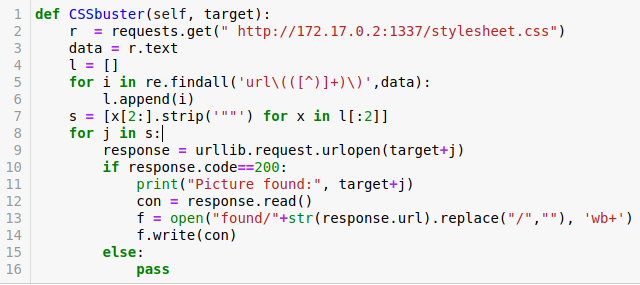
\includegraphics[scale=0.5]{data/cssbuster.png}
\end{center}
\begin{center}
 Codebeispiel 4: CSSbuster
\end{center}
Die Funktion findet alle in CSS Dateien hinterlegten Bilder.
\newpage
\subsection{Selenium Browser Angriff}
Bei diesem Angriff sollen automatisiert möglichst alle Seiten der Webanwendung besucht werden. Zudem sollen Funktionalitäten wie Formulare befüllt und abgeschickt werden.
\begin{center}
 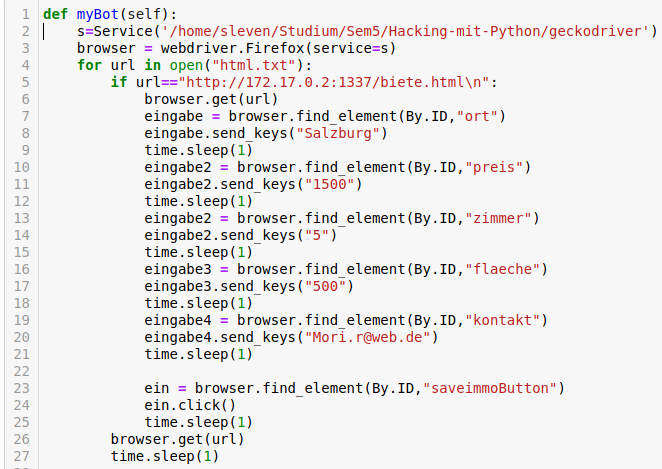
\includegraphics[scale=0.5]{data/bot.png}
\end{center}
Anfangs wird der entsprechende Treiber für den Firefox browser eingeladen(vgl. Zeile 2-3). Anschließend wird über die zuvor angelegte Datei mit den Html Dokumenten iteriert und jeweilige Seiten geöffnet. In der Seite 'biete.html' werden zudem Formulardaten eingetragen und abgeschickt(vgl. Zeile 7-23).
\newpage
\subsection{SSH Angriff}
Hierbei sollen Admin-Schnittstellen angegriffen und Kompromitiert werden.
Die Webanwendung wird über eine SSH Schnittstelle gewartet. Nun  wird versucht anhand eines Wörtbuch Angriffes an die Anmeldedaten zu gelangen.
\begin{center}
 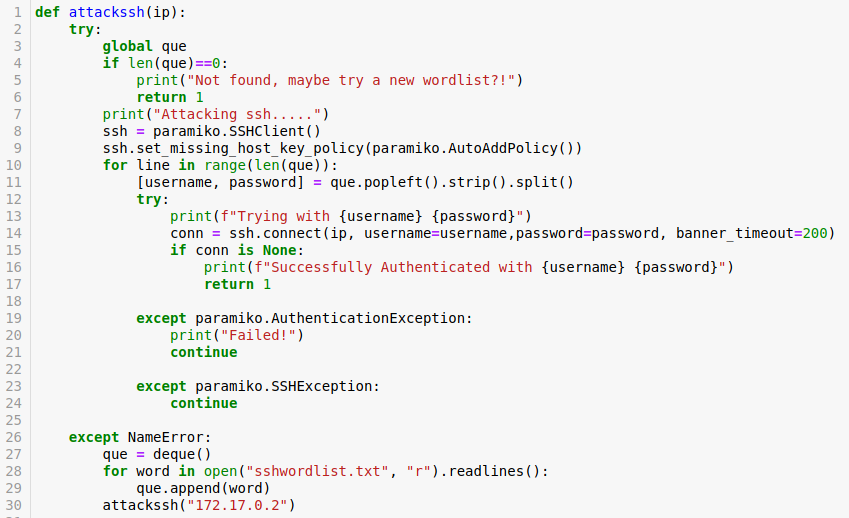
\includegraphics[scale=0.5]{data/ssh.png}
\end{center}
Anfangs wird eine que angelegt, die in einer Exception befüllt wird(vgl. Zeile 28). Die Funktion wird anschließend erneut aufgerufen und es wird überprüft ob die que leer ist. Nun wird die Paramiko Biblothek aufgerufen(vgl. Zeile 8). Diese bietet SSH Implementierungen für client und serverseitige Funktionalitäten. Ab Zeile 11 wird Username und Passwort aus der que ausgelesen und entsprechen formatiert. Nun wird versucht eine Verbindung mit den übergebenen Anmeldedaten herzustellen(vglt. Zeile 14). Ist die verbidnung erfolgreich, werden Nutzername und Passwort ausgegeben(vgl. Zeile 16), sowie das Programm gestoppt. Im gleichen Schleifendurchlauf werden zudem exceptions abgefangen. Die Funktion findet das Passwort und gibt es aus.\\
\begin{center}
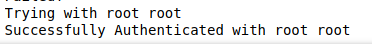
\includegraphics[scale=0.5]{data/success.png}
\end{center}
\subsection{Schadsoftware}
Nun soll über die erlangten Zugangsdaten eine Schadware auf den Opfer Server geladen werden, die ein Defacement der Seite umsetzt und zudem die Zugangsdaten der Schnittstelle ändert.
\end{document}
